\documentclass[12pt, letterpaper]{article}

\usepackage{graphicx}

\title{How2HotShot: A Guide to Operating the Hot Shot Electric Boiler for Teaching Assistants}
\author{Joshua Holbrook}

\begin{document}

\maketitle

\section{Introduction}

\begin{figure}
\label{fig:boiler}
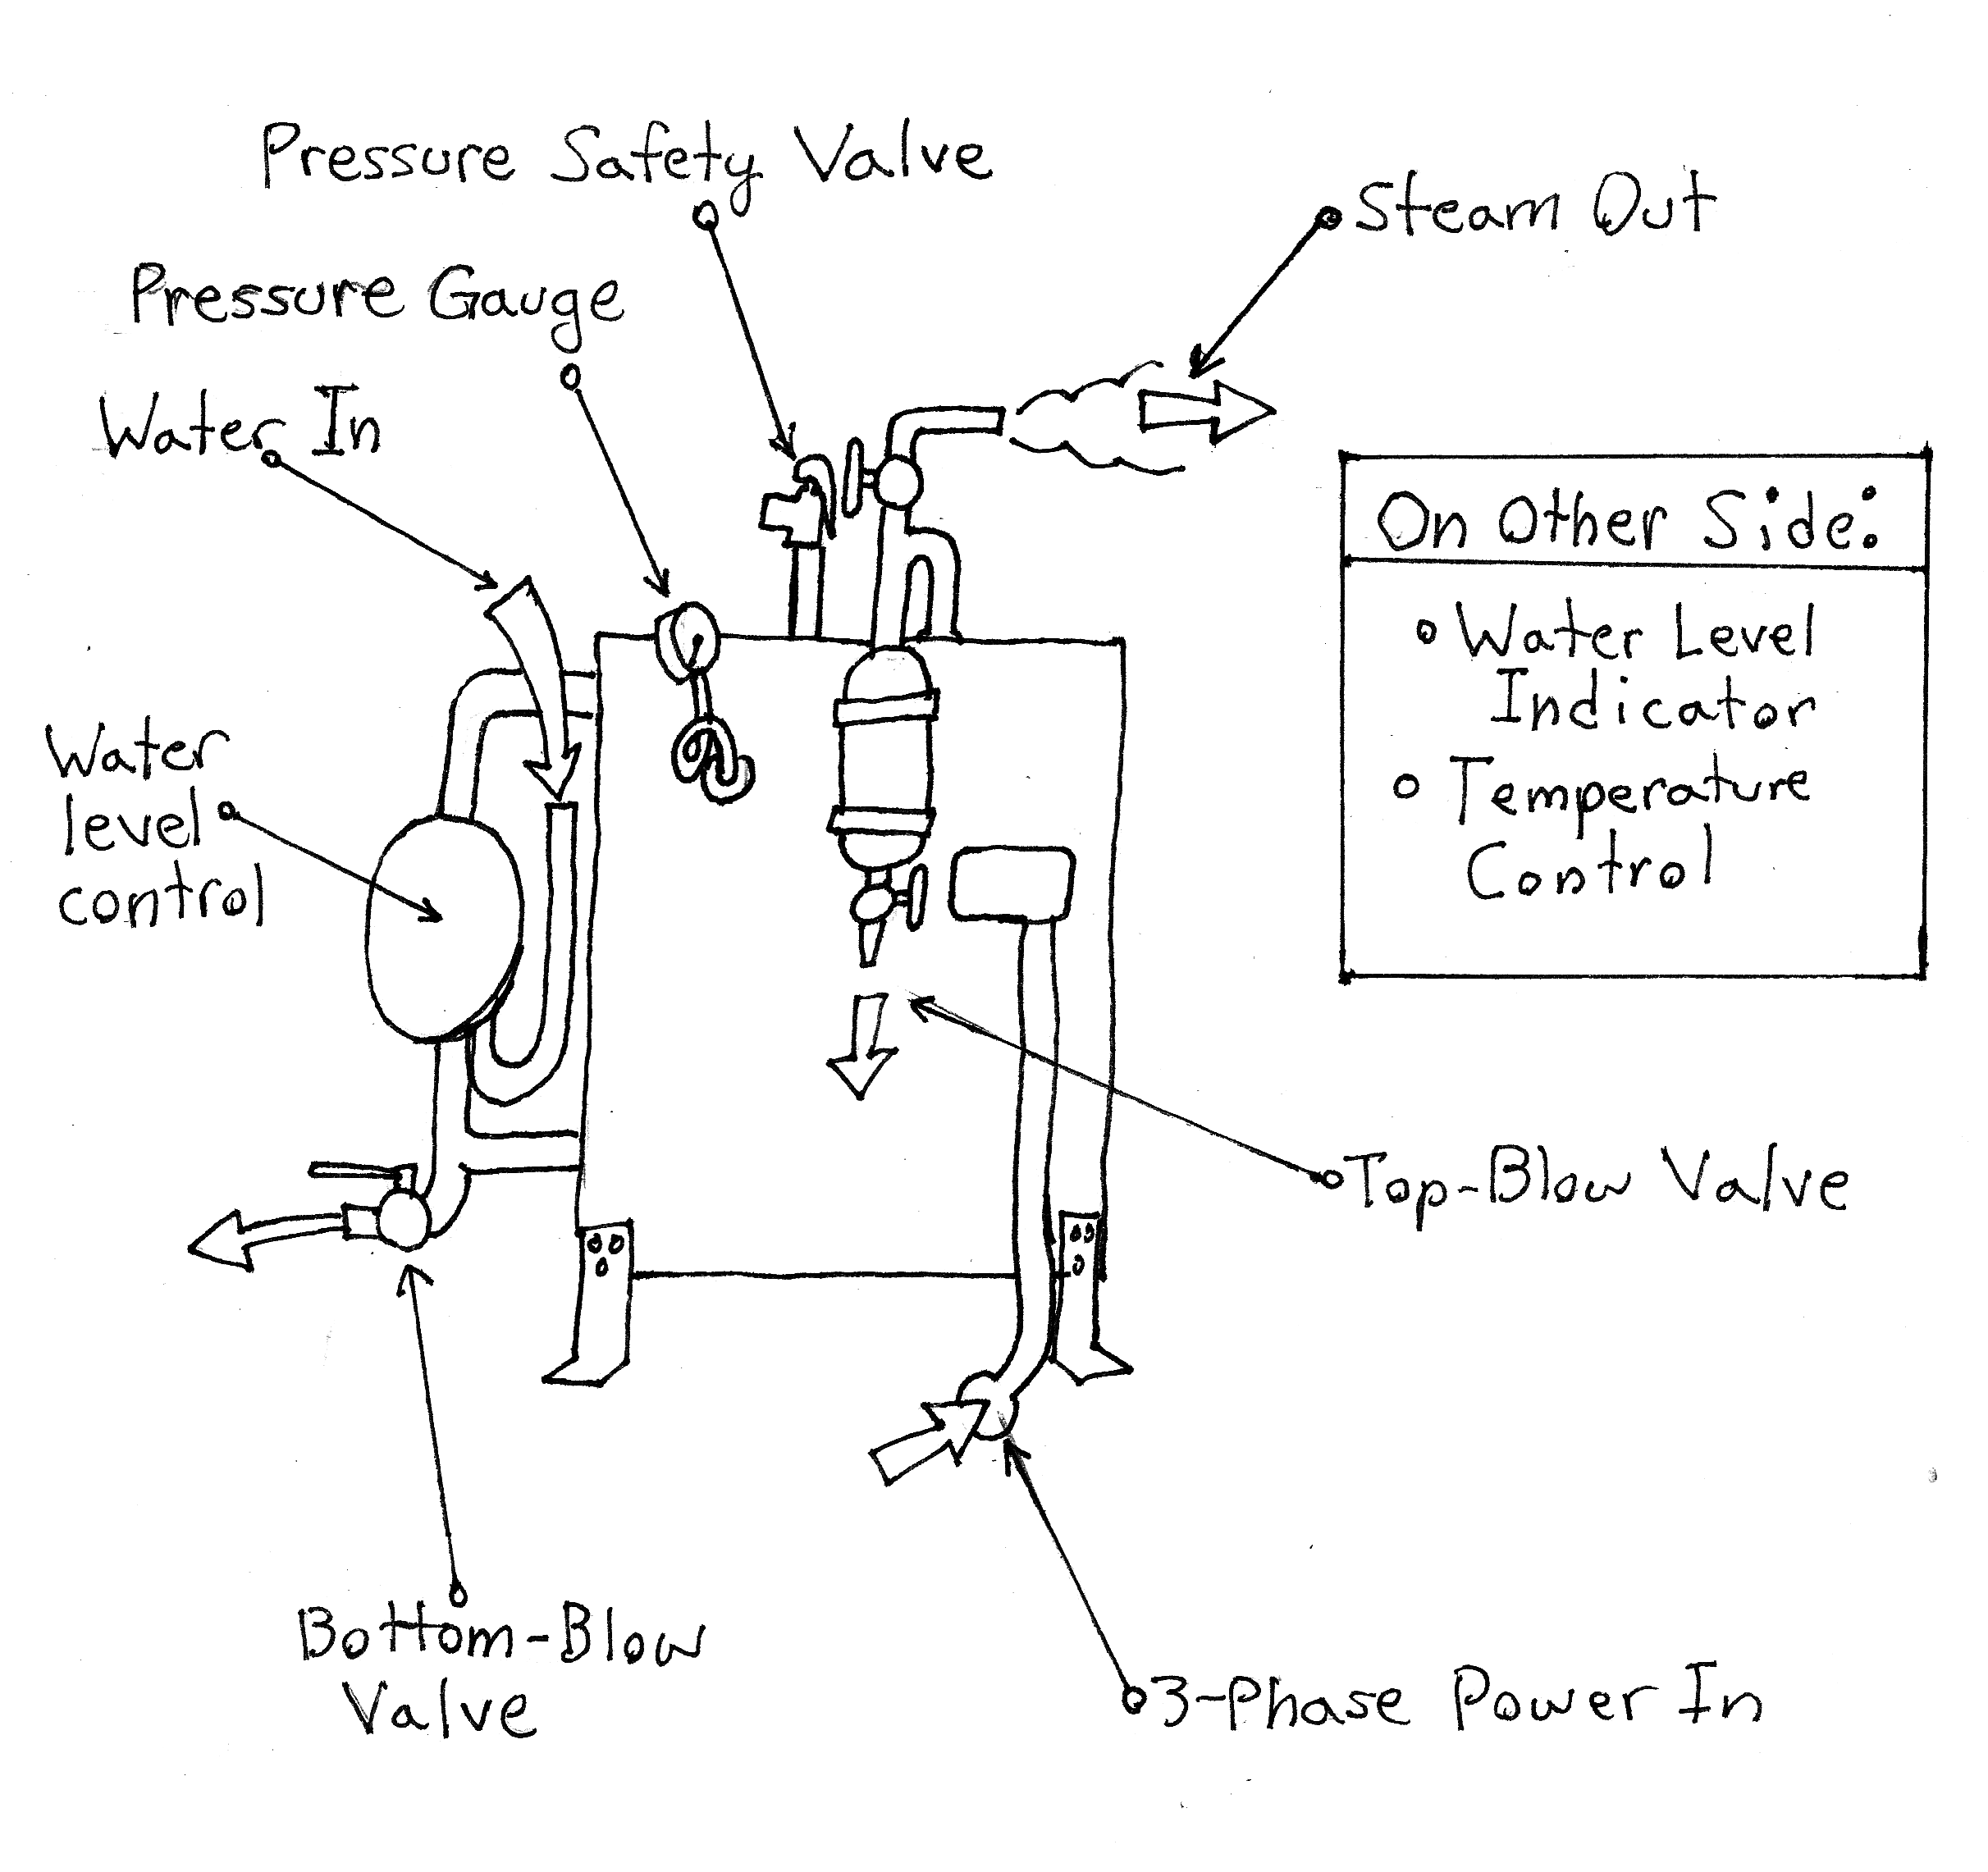
\includegraphics[width=0.9\textwidth]{boiler}
\caption{A sketch of the Hot Shot boiler, with important parts labelled.}
\end{figure}

The boiler, conceptually, is actually quite simple. It uses electric heating elements to boil water. Water is supplied with a hose, and hot steam comes out.

The water level is controlled by what is labelled as the ``water level control'' in Figure \ref{fig:boiler}. Think of it kinda like a toilet float. The water level should be visible on the glass tube on the front of the boiler, at roughly \(1/2\) to \(2/3\) full.

The top-blow and bottom-blow valves (also labelled in Figure \ref{fig:boiler}) are meant for clearing out steam/condensate and water, respectively, from the boiler. In practice, only the bottom-blow valve is used.

Unlike many boilers, the Hot Shot is temperature-controlled. If one wants a given pressure (a common occurrence), one should consult steam tables and assume saturated steam. For example, 15 psig is equivalent to about 300 degrees Fahrenheit, which happens to be around the upper end of the Hot Shot's capabilities.

\section{Set-Up}

\begin{enumerate}

\item Hook the water inlet to a water source.

\item Open the steam outlet. This allows air to escape so that the boiler can fill more quickly.

\item Turn on the water, and wait for the device to fill.

\item Plug in the boiler and turn the temperature knob to the desired temperature.

\item It's not critical, but by my estimation, keeping the steam outlet closed while the boiler reaches temperature will make the process go faster.

\end{enumerate}

\section{Operation with the Temperature in Rods Apparatus}

Operating the steam boiler---that is, utilizing the steam---is a process that depends somewhat on the device that's being supplied. In this case, the Hot Shot is used to run a ``temperature in rods'' lab.

\begin{enumerate}

\item Hook the device to the boiler using a washing machine hose.

\item Keep the condensate drain valve on the apparatus open.

\item Turn the boiler steam outlet valve open \emph{slowly}.

\item By adjusting the boiler steam outlet valve and the condensate drain valve, try to get the steam pressure at 15 psig, with ``spittle'' coming from the drain valve and the pressure valve happily chattering.

\end{enumerate}

\section{Tear-Down}

\begin{enumerate}

\item Allow the boiler to cool.

\item Connect a hose from the bottom-blow valve to a drain.

\item Open the steam outlet valve, the bottom-blow valve, and the water inlet valve.

\item Flush water through the boiler until it runs clear. Initially, it will be rusty and mucky.

\item Once the water runs clear, turn off the water inlet valve and allow the boiler to drain completely.

\item Disconnect everything and put the hoses away. You're done!

\end{enumerate}

\end{document}
